% Chapter 2

\chapter{Methods and Models} % Main chapter title

\label{Chapter2} % For referencing the chapter elsewhere, use \ref{Chapter1} 

\lhead{Chapter 2. \emph{Methods and Models}} % This is for the header on each page - perhaps a shortened title

%----------------------------------------------------------------------------------------


\textit{Graph theory} is a mathematical field applicable to a considerable diversity of complex systems such as markets, ecosystems, computer circuits, and gene-gene interactions \citep{XYZ09}. A graph is defined as an ensemble of vertices (nodes) that are linked with edges. If the edges connect the nodes in a specified direction, the graph is referred to as \textit{directed}, otherwise \textit{undirected}. Moreover, the edges can be assigned a weight yielding a \textit{weighted} graph. A graph with edges of uniform weight is called an \textit{unweighted} graph.

\textit{Network science} incorporates graph theory applied on a   
distinct complex domain. Unlike classical graph theory, network science primarily deals with real life networks that are large and complex - neither uniformly random nor ordered \citep{RUB10}. The neuro-anatomical and neuro-physiological data sets derived from  DW-MRI and fMRI-BOLD techniques can be constructed as such large-scale complex brain graphs that are undirected and unweighted. Nodes in large-scale brain networks usually represent brain regions, while edges represent anatomical, functional or effective connections \citep{XYZ94}. 


A brain network can be statistically described in terms of its topology, i.e. solely in terms of its connectivity and independently of spatial positions of nodes and edges. Topological measures described in previous studies capture local and global properties of a network, e.g. local and global efficiency, clustering coefficient, transitivity and small-worldness \citep{LAT01, WAT98, NEW03, HUM08}.


Methods of graph theory applied to structural and functional systems have shown that both share typical features of many complex networks \citep{BUL09, RUB09, HEU11, VUK14}. However, the essential features of brain's connectivity still remain ambiguous both for functional and structural maps. This project aims to investigate whether the brain does not behave as a completely random circuitry. This idea will be tested by comparing brain graphs to the randomized networks as it was previously noticed by Bullmore and Bassett \citep{BUL11a}. The majority of random graphs here are inspired by  Erd\H{o}s-R\'{e}nyi type random networks and the configuration model. 
 

In this section, the construction of brain graphs based on empirical functional connectivity matrix (FCM) and anatomical connectivity matrix (ACM) will be first introduced. Then, the topological characteristics of all graphs will be statistically measured and those topological measures will be interpreted neuro-biologically. In particular, it is aimed to explore under which conditions that brain network topologies distinguish from random networks. This approach is expected to provide a deeper insight into the underlying process involved in the observed functional and structural brain connectivity. 


\section{Empirical functional and anatomical connectivity matrices}

The functional-magnetic-resonance-imaging (fMRI) is a widely used method to detect the blood-oxygen-level-dependent (BOLD) contrast in the brain. The fMRI-BOLD contrast is used to interpret the neuronal activity in the respective voxel, which can be considered as a rectangular volume in brain defined for the imaging studies. The ongoing firing activity of neurons requires energy and it is supplied by neighboring blood cells via oxygen and glucose release into the nerve cells. The deviations in deoxygenation level, cerebral flow and volume in blood vessels due to neuronal activity, known as \textit{hemodynamic process}, cause a change in the detected fMRI-BOLD signal strength. The functional connectivity matrix (FCM) represents correlation coefficients of these fMRI-BOLD signals detected from the pre-defined brain regions with voxels. 

The resting state empirical FCM used in this project is obtained from the \textit{1000 Functional Connectome Project} website \url{http://www.nitric.org/}). The human brain is segmented into $N=90$ cortical and sub-cortical regions according to the Tzourio-Mazoyer brain atlas with the automated anatomical labeling (AAL) template  \citep{TZO02}, such that regions with index $n=\{1,2,...,45\}$ lie on the right hemisphere, whereas $n=\{46,47,...,90\}$ on the left. The fMRI-BOLD activity is measured from all voxels in an AAL region for 7.5 min of acquisition time. Once the fMRI-BOLD mean time-series are obtained for all AAL regions, then the FCM is obtained by calculating the Pearson correlation coefficients of timeseries between all pairs in 90 AAL regions. Therefore the size of FCM is $N\times N = 90 \times 90$.  To be more precise, BOLD-fMRI signal is averaged for the same subject over voxels in an AAL region, and FCM is averaged over all subjects at the end. 

The diffusion-weighted magnetic-resonance-imaging (DW-MRI) technique estimates the anatomical connection probabilities among brain regions by investigating the diffusion direction of water molecules within a voxel. The direction of the fiber tracks in white matter depends on the diffusion pattern of water molecules. A DW-MRI experiment approximates the existence of a fiber track between regions of interest. The anatomical connectivity matrix (ACM) used in this project is obtained from the study of Iturria-Medina et. al. \citep{ITU08} and it is based on the same $N=90$ AAL regions as in the FCM described above. The size of ACM is also $NXN = 90X90$, and each value reveals the probability of 2 AAL regions being connected via axonal fibers. 
  
\begin{figure}[htbp]
 
  \centering
	 \includegraphics[width=0.49\textwidth]{Figures/FCM.eps} 
	 \includegraphics[width=0.49\textwidth]{Figures/ACM.eps} 
	
    \rule{35em}{0.5pt}
  \caption[Empirical FCM and ACM]{Empirical functional and anatomical connectivity maps of human cortex, FCM obtained from fMRI-BOLD technique (on the left) and ACM obtained from DW-MRI (on the right). The colorbars exhibit correlation coefficients and probability values in FCM and ACM, respectively. }
  \label{fig:Empirical FCM and ACM}
 	
\end{figure}  

 
\begin{figure}[htbp]
 
  \centering
	 \includegraphics[width=0.49\textwidth]{Figures/FCM_brain.eps} 
	 \includegraphics[width=0.49\textwidth]{Figures/ACM_brain.eps} 
    \rule{35em}{0.5pt}
  \caption[Empirical FCM and ACM in cortex]{3D sagittal visualization of FCM and ACM on the human cortex with the \textsc{BrainNet Viewer} \citep{XYZ13}. } 
  \label{fig:Empirical FCM and ACM in cortex}
 	
\end{figure} 

Figure 2.1 represents empirically captured FCM and ACM. All correlation coefficients in FCM appear in the range [0,1] as well as all probability values in ACM. Both matrices are symmetric. A correlation value close to 1 in FCM indicates that the quantified functional activities of corresponding nodes highly resemble each other. A probability value close to 1 in ACM demonstrates that corresponding nodes are most likely connected by fiber tracks in white matter. Although some node pairs are not anatomically coupled at all in ACM (cold colors), they could be functionally coupled in FCM (hot colors).    

FCM and ACM are embedded in human cortex in Figure 2.2 \citep{XYZ13}. All nodes are presented with equal size and black color independent of their topological properties. However, edges have different thickness and color distribution according to correlation coefficients and probability values with respect to FCM and ACM. 
 
   
\section{The Brain Graph}

The brain graphs considered here are derived from two sets of empirical brain connectivity maps: FCM and ACM obtained from fMRI-BOLD and DW-MRI techniques, respectively. Those data sets represent measurements from $N=90$ cortical and sub-cortical regions labeled with AAL, represented by nodes in the graph. The nodes can be connected to each other by means of "edges". If the graph is constructed on the FCM, edges are interpreted as correlation strengths between the functional BOLD activity of two nodes. If the graph is built on the ACM, an existing edge is considered as the probability of two nodes to be structurally connected by fiber tracks in white matter.

The brain graphs in this project are generated through binarizing the functional connectivity matrix (FCM) and anatomical connectivity matrix (ACM). Binarization here means converting all the values in a given matrix into 1's and 0's via thresholding. Because of the nature of their definition, both empirical data sets have values between 0 and 1, reflecting a correlation strength in case of FCM or a probability value in case of ACM. We arbitrarily define a threshold value $r$ for the strength of correlations in FCM. Then, the values greater and equal to $r$ are assigned the value 1, while others are set to 0. This thresholding is applied by means of the strength of probability value, $p$, for the ACM. The binarized matrix is the basis of brain graph construction, and it is commonly known as \textit{adjacency matrix}. The \textsc{Networkx} software package in \textsc{PYTHON} is used to built graphs given adjacency matrices. Neither the direction of functional or anatomical connectivity between nodes, nor any other values apart from 0 and 1  are encoded in the adjacency matrices,  so that the resulting graphs are considered as "undirected" and "unweighted". In other words, all existing edges are thought to be of uniform weight and nodes interact both ways along an edge connecting them. 

\begin{figure}[htbp]
 %\begin{tabular}{cc}
  \centering
	 \includegraphics[width=0.45\textwidth]{Figures/FCM.eps} 
	 \includegraphics[width=0.45\textwidth]{Figures/Sample_Adj.eps} 
	\includegraphics[width=0.45\textwidth]{Figures/Sample_Adj_brain.eps}  
   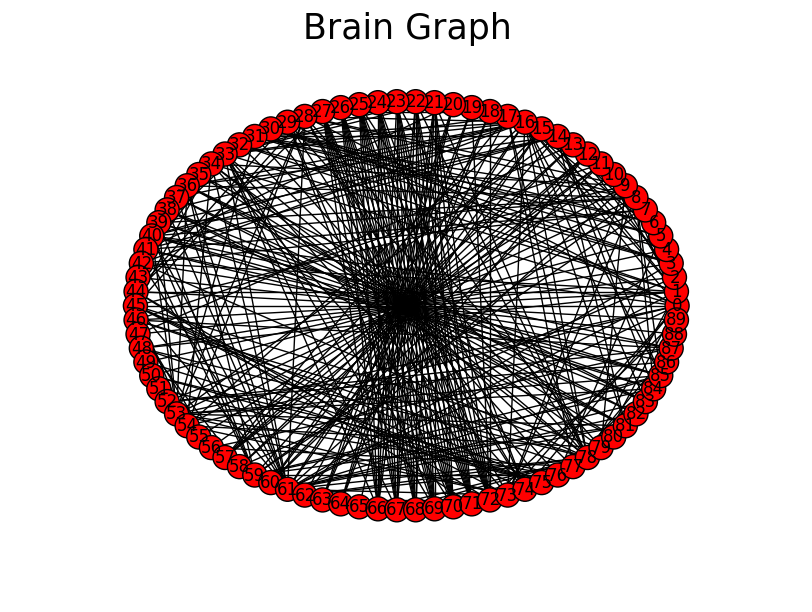
\includegraphics[width=0.45\textwidth]{Figures/brain_graph.png}      

    \rule{35em}{0.5pt}
  \caption[Binarizing via thresholding]{How to build a brain graph : The empirical data matrix derived from fMRI-BOLD technique (on the upper left) is binarized via a threshold value $r=0.55$ and its corresponding adjacency matrix (on the upper right). The black spots represent 1's indicating edges between nodes, whereas the white squares represent 0's implying no edge at all. The adjacency matrix is embedded on human cortex axially (on the lower left) with \textsc{BrainNet Viewer} \citep{XYZ13} and the brain graph derived from the adjacency matrix with \textsc{NETWORKX} (on the lower right).}
  \label{fig:Binarizing via thresholding}
 %\end{tabular}	
\end{figure}

Figure 2.1 illustrates the exemplary construction of a brain graph from the FCM. All correlation values among the cortical and sub-cortical regions in the empirical fMRI-BOLD data lie between 0 and 1. 3D axial cortex visualization represents only the existing edges with black edges among the nodes. The adjacency matrix (AM) is filled out only with 1's and 0's indicating functionally connected and unconnected nodes, whose correlated BOLD activity is equal to or greater than $r=0.55$. The algorithm \textsc{Networkx} builds the corresponding graph of an adjacency matrix. The AM obtained from an ACM would look similar, but would represent the probability of two nodes to be anatomically connected above a predefined threshold $p$. 

The following sections will cover randomization methods reshuffling the brain graphs and introduce some of the topological concepts characterizing brain graphs as well as random networks.



\section{Randomization Methods}





\subsection{Erd\H{o}s-R\'{e}nyi Type Randomization}

Given a total number of nodes $N$, Paul Erd\H{o}s and Alfr\'{e}d R\'{e}nyi produced an undirected graph $G(N,P)$, in which the presence of any edge between two nodes is assigned a probability $P$. 
The average total number of edges $L$ in an  Erd\H{o}s-R\'{e}nyi type random graph is $\binom {N} {2}P$, with a binomial distribution for the number of edges per node.

New randomization techniques arise through modifying the Erd\H{o}s-R\'{e}nyi method, e.g. given $N$ and $L$, a graph $G(N,L)$ can be picked uniformly random out of set of all potential graphs having $N$ nodes and $L$ edges. The probability for a graph to be picked among all the others is $\frac{L}{\binom {N}{2}}  $. One can study the various aspects of $G(N,P)$ and $G(N,L)$ even more detailed, but for the sake of simplicity, Erd\H{o}s-R\'{e}nyi model will not discussed further here.

\begin{figure}[htbp]
 %\begin{tabular}{cc}
  \centering
	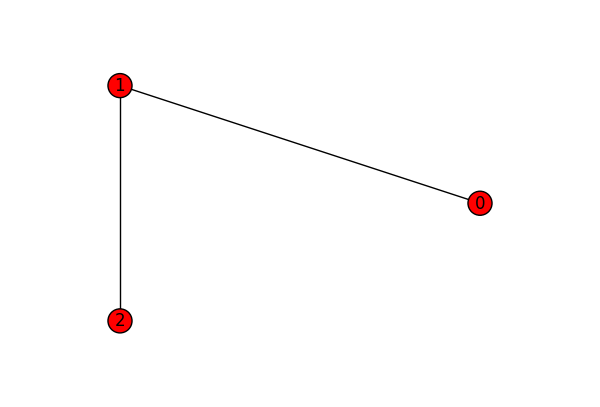
\includegraphics[width=0.30\textwidth, height=40mm]{Figures/f1.png}  
	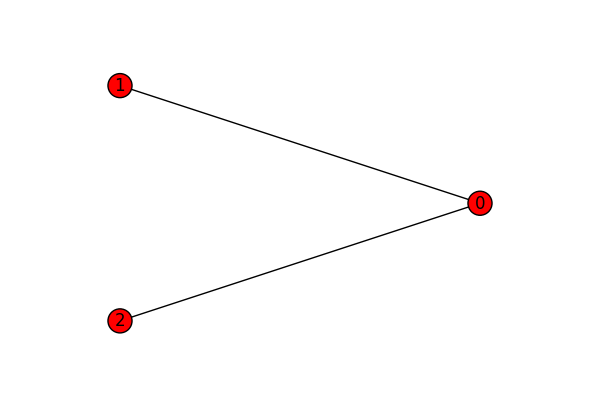
\includegraphics[width=0.30\textwidth, height=40mm]{Figures/f2.png} 
    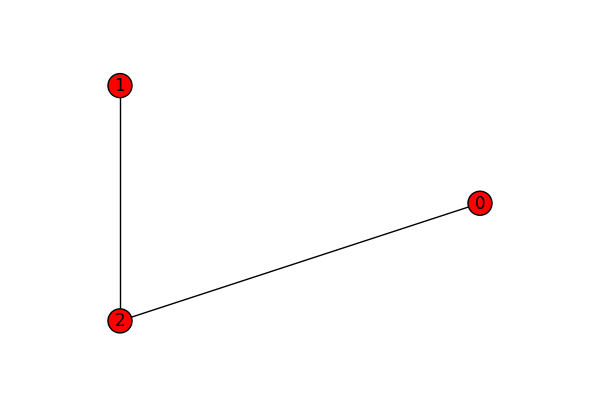
\includegraphics[width=0.30\textwidth, height=40mm]{Figures/f3.png}

    \rule{35em}{0.5pt}
  \caption[Erdos-Renyi Example]{An illustration of the set of all $G(N,L)$ type random graphs with $N=3$ and $L=2$.}
  \label{fig:Erdos-Renyi Example}
 %\end{tabular}	
\end{figure}

Figure 2.2 illustrates all possible graphs having 3 nodes and 2 edges. One of those 3 simple graph is chosen uniformly random for the $G(N,L)$ randomization type, so that each graph is chosen with probability $P=\dfrac{1}{3}$.  

The $G(N,L)$ type randomization is the first method used to derive random graphs from the adjacency matrices of FCM and ACM in this project. Both matrices have $N=90$ nodes, however $L$ changes for each brain graph according to the applied threshold level and therefore is always recalculated. 

\subsection{Double-Edge-Swap Type Randomization}

The \textit{degree} $k_i$ of a node $i$ is defined as the number of edges connected to that node. The double-edge-swap method manipulates a given graph by swapping two existing edges among four nodes, while keeping the node degrees fixed. 


\begin{figure}[htbp]
 %\begin{tabular}{cc}
  \centering
	\includegraphics[width=0.32\textwidth, height=50mm]{Figures/G1_swap.eps}  
    \includegraphics[width=0.32\textwidth, height=50mm]{Figures/G2_swap.eps}  
	\includegraphics[width=0.32\textwidth, height=50mm]{Figures/G3_swap.eps} 
    \rule{35em}{0.5pt}
  \caption[Double-Edge-Swap Example]{Swapping edges between 2 paired nodes}
  \label{fig:Double-Edge-Swap Example}
 %\end{tabular}	
\end{figure}

Figure 2.3 illustrates randomly chosen double edges in a sample graph to be swapped. After the existing edges are removed, the new pair of nodes are rewired. The degree of each node is the same before and after swapping; degrees of nodes $k_1 = 1$, $k_2=1$, $k_3=1$, $k_4=1$ are all fixed in each graph. Although the randomly constructed graphs with the double-edge-swap method are expected to have same degrees, the latter is not a unique property identifying a graph.

The \textit{degree distribution} is the probability distribution of node degrees over the whole graph. Conservation of each $k_i$ preserves the degree distribution, however, preserving degree distribution does not guarantee to fix $k_i$ values. We will discover in the next section how to preserve degree distribution by altering node degrees.

\subsection{Preserved-Degree-Distribution Type Randomization}

The preserved-degree-distribution method randomizes a given network by adding-removing or rewiring its edges randomly while recovering its degree distribution $P(k)$. The idea is to reassign edge indices in the graph, meaning that the degree of individual nodes may change. P(k) is defined with the following equation,

\begin{equation}
P(k) = \sum_{k' \geq k} p(k')
\end{equation}

where $p(k')$ is the probability of a node to have degree number $k'$ \citep{BAR99a}.


\begin{figure}[htbp]
 %\begin{tabular}{cc}
  \centering
	\includegraphics[width=0.45\textwidth, height=60mm]{Figures/G_degree_dist_1.eps}  
	\includegraphics[width=0.45\textwidth, height=60mm]{Figures/G_degree_dist_2.eps}    
    \rule{35em}{0.5pt}
  \caption[Degree Distribution 2D Example]{Reconstruction of a given graph (on the left) with degree-distribution-preservation model (on the right). $k_i=\{3,1,1,1\}$ in the original graph and $k_{i}=\{1,0,1,3,1\}$ in the randomized graph. }
  \label{fig:Degree Distribution Example}
 %\end{tabular}	
\end{figure}

The algorithm is thought to add-remove new nodes to a given graph while preserving $P(k)$ as shown in Figure 2.6. However, we randomize our brain graph with a conserved total number of nodes $N$ as well as $P(k)$. The figure is given only for a better visualization in order to distinguish preserved-degree-distribution randomization method and configuration model randomization, which will be introduced in the next section.

\begin{figure}[htbp]
 %\begin{tabular}{cc}
  \centering
	\includegraphics[width=\textwidth]{Figures/G_degree_dist.eps}  
    \rule{35em}{0.5pt}
  \caption[Degree Distribution 3D Example]{Heat maps for degree distributions of the brain graph obtained from FCM (on the left), and of the randomized graph with preserved-degree-distribution tool (on the right). Colorbars are in logarithmic scale with lower and upper limits : $[\log_{10} {10}^0 , \,  \log_{10} {10}^1]$}
  \label{fig:Degree Distribution 3D Example}
 %\end{tabular}	
\end{figure}

$P(k)$ is a global topological measure for a network, it can be illustrated over all nodes in the whole graph as in Figure 2.7. Node indexes are labeled on $x$ axis on heat maps, threshold $r$ values for adjacency matrices are given on $y$ axis. The preserved-degree-distribution method generates successfully a random graph with the same $P(k)$ as in the brain graph. 


\subsection{Configuration Model Randomization}

The \textit{degree sequence} of a graph is either its ascending or descending sequence of node degrees. The configuration model generates a random graph with a given degree sequence. The direct implementation of this model is to assign edges to the nodes randomly until the desired degree sequence is matched. The resultant random graph is expected to be a node-index-shuffled version of the original graph. However, these algorithms are non-trivial due to the occurrence of self-loops (node is connected to itself) and parallel edges (multiple edges connecting two nodes), which are both undesirable graph properties in this project. 

\begin{figure}[htbp]
 %\begin{tabular}{cc}
  \centering
	\includegraphics[width=0.45\textwidth, height=60mm]{Figures/G_config_1.eps}  
	\includegraphics[width=0.45\textwidth, height=60mm]{Figures/G_config_2.eps} 
    \rule{35em}{0.5pt}
    \caption[Degree Sequence Definition]{The degrees of the nodes in the original graph (on the left): $k_0 = 2$, $k_1 =1$, $k_2=2$, $k_3=3$ and that of the randomized graph (on the right) : $k_0 = 3$, $k_1 =2$, $k_2=1$, $k_3=2$. The degree sequence in non-increasing order in both graphs : $\{3,\,2,\,2,\,1\}$}
  \label{fig:Degree Sequence Definition}
 %\end{tabular}	
\end{figure}

Figure 2.8 points out the relevance of the degree sequence to the node degrees. Moreover, one should not confuse degree distribution and degree sequence.   

The configuration model variant used here is the expected-degree-graph method, which excludes self-loops and parallel edges. This algorithm receives the list of the expected degree sequence as an input $(k_u, k_v, k_m, k_l, ...)$, and assigns edges between nodes with a predefined probability $P_{uv}=\dfrac{k_u k_w}{\sum_{i}k_i}$. This method does not guarantee to construct graphs with exactly the same given degree sequence but with the closest possible sequence.  



 
\subsection{Partial Randomization}
 
The partial randomization method  reconstructs a graph (say A) with partial rewirings with respect to a second graph (say B) while keeping the degree distribution the same as in A. The analogy of this algorithm is to perform rewirings in the adjacency matrix of A, while avoiding any edge generation which already exist in the B. In other words, the choice of edges to be performed rewirings in A is limited with respect to the B. 

In this project, the functional connectivity (FC) adjacency matrix is partially rewired with respect to the anatomical connectivity (AC) adjacency matrix.  This means doing such rewirings among the nodes in FCM only if these nodes are not structurally connected in the brain with probability above a given value. The same procedure is done to randomize AC adjacency matrix partially with respect to FC adjacency matrix.  This time nodes in ACM can be linked only if they are not functionally correlated above a given threshold.   

\begin{figure}[htbp]
 %\begin{tabular}{cc}
  \centering
	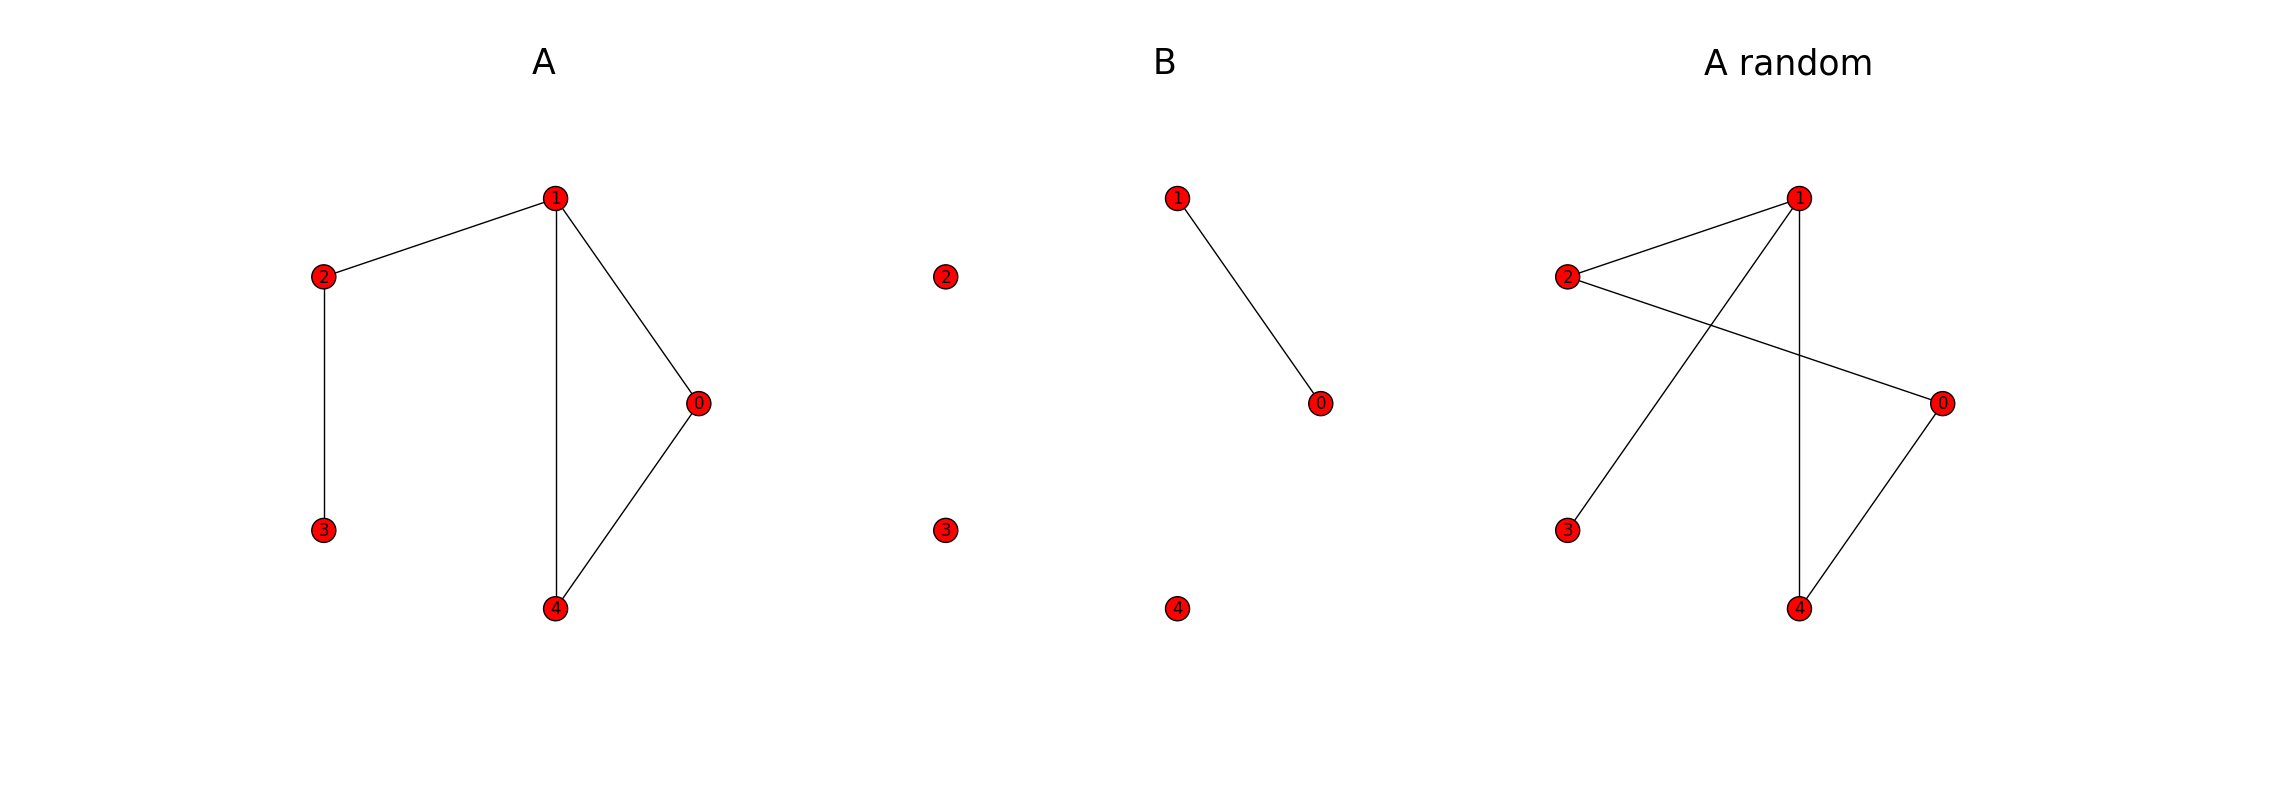
\includegraphics[width=\textwidth, height=55mm]{Figures/p1.png}  
    \rule{35em}{0.5pt}
    \caption[Partial Randomization Example]{Graph A is performed a partial randomization with respect to graph B. While the partial randomization tool rewires edges in A, it avoids creating such edges that exist in B.}
  \label{fig:Partial Randomization Example}
 %\end{tabular}	
\end{figure}

Representative graphs $A$ and $B$ in Figure 2.9 can be thought as FCM and ACM, respectively. In this case, $A \,\, random$ is the partially randomized graph of FCM with respect to ACM.


The brain graph and randomly generated graphs will be identified in terms of their topological properties in the following sections. For simplicity the abbreviations are introduced in the table below. 

\begin{table}[h]
\begin{center}
\caption[Abbreviations]{Abbreviations for the brain graph and the randomly constructed graphs. }
\begin{tabular}{ l | c | r }
  Abbreviation & Description & method \\
  \hline  \hline                     
  R0 & the brain graph						  & \textsc{networkx} \\ \hline
  Ra & Erd\H{o}s-R\'{e}nyi, G(N,L)            & \textsc{networkx} \\ \hline
  Rd & double-edge-swap            			  & \textsc{networkx} \\ \hline
  Rh & preserved-degree-distribution		  & \textsc{BCT} 	 \\ \hline  
  Rg & configuration model       			  & \textsc{networkx} \\ \hline
  Rk & partial randomization            	  & \textsc{BCT} 	 \\ \hline  
  \hline  
\end{tabular}
\label{table:Abbreviations}
\end{center}
\end{table}	

\section{Network Characterizations}

\subsection{Network Density}
The \textit{average degree} $\langle k \rangle$ of a network is proportional to the ratio of total number of edges $L$ to total number of nodes $N$ in a graph, 

\begin{equation}
\langle k \rangle = \frac{2L}{N}.
\end{equation}

It should be noted that in order to not count each edge twice, the total number of edges is divided by $N/2$ instead of $N$. The \textit{density} $D$ of a network is a scaled version of average degree measurement. It is formulated as the ratio between $L$ and maximum number of possible edges ${N \choose 2}$,

\begin{equation}
D = \frac{2L}{N(N-1)}.
\end{equation}	

The measure of network density can be referred to as the total \textit{wiring cost} of the network \citep{RUB10}. The degree, average degree and network density are key scalar measures to characterize the topology of a network. There is for instance clinical evidence that reductions in nodal degree are associated with greater severity of local amyloid deposition in patients with Alzheimer's disease \citep{XYZ2009}. 

\begin{figure}[htbp]
 %\begin{tabular}{cc}
  \centering
	\includegraphics[width=0.48\textwidth, height=55mm]{Figures/Network_Density_Fnc.eps}
	\includegraphics[width=0.48\textwidth, height=55mm]{Figures/Network_Density_Stru.eps}  
    \rule{35em}{0.5pt}
    \caption[Network Density]{Network density of the brain graphs and random graphs of FCM (on the left) and ACM (on the right). The abbreviations are chosen as described in Table 1.}
  \label{fig:Network Density}
 %\end{tabular}	
\end{figure}


The network density $D$ can be considered a probability for all graphs in corresponding threshold $r$ and $p$ ranges. The random networks are built in such ways that they have the same number of nodes and almost the same $D$ as in the brain graphs. However, the $D$ is not a unique metric identifying a network.

All networks for FCM and ACM are densely connected for low $r$ and $p$. For the brain graph and randomized graphs of FCM, $D$ decreases sigmoidally with $r$. In comparison, $D$ decreases slower with $p$ for ACM graphs. It should be noted that all graphs have almost the same $D$ values. 

Functional networks are likely to be denser than anatomical networks, as they will typically contain numerous connections between anatomically unconnected regions \citep{DAM09}. 

\subsection{Average Clustering Coefficient}
    
The \textit{average clustering coefficient} $C$ of a network is calculated through individual clustering coefficients $C_i$ of single nodes,

\begin{equation}
C = \frac{1}{n} \sum\limits_{i\epsilon N}C_i = \frac{1}{n}\sum\limits_{i\epsilon N} \frac{2t_i}{k_i(k_i -1)} .
\end{equation} 

where $t_i$ is the number of triangles around node $i$ and $k_i$ is the degree of node $i$ \citep{WAT98}. The clustering coefficient is a measure of segregation, that is the ability for specialized processing to occur within densely interconnected groups of brain regions \citep{RUB10}. It reveals how the individual nodes in a graph cluster together; how many neighbors of a node are neighbors of each other. 

\begin{figure}[htbp]
 %\begin{tabular}{cc}
  \centering
	\includegraphics[width=0.48\textwidth, height=55mm]{Figures/Clustering_Coefficient_Fnc.eps}
	\includegraphics[width=0.48\textwidth, height=55mm]{Figures/Clustering_Coefficient_Stru.eps} 
    \rule{35em}{0.5pt}
    \caption[Clustering Coefficient]{Average clustering coefficient of the brain graphs and random graphs of FCM (on the left) and ACM (on the left). }
  \label{fig:Clustering Coefficient}
 %\end{tabular}	
\end{figure}

The clustering coefficient $C_i$ of a node $i$ is a measure of local connectivity and is highly correlated with the local efficiency of the information transfer \citep{LAT01}. The $C_i$ is formulated as the ratio of $t_i$ over all possible edges of the node $i$; ${k_i \choose 2} $. The average clustering coefficient $C$ is a normalized version of $C_i$ for the whole network, yielding now a global property. All $C$ values are between 0 and 1. Figure 2.7 shows that at lower binarization thresholds, nodes tend to cluster more due to higher number of existing edges. The empirically obtained brain networks of FCM and ACM have the highest $C$ compared to random graphs. The local information transfer seems to be more efficient in the brain graphs.  The randomized graphs of ACM $Ra$, $Rd$, $Rh$ and $Rk$ share more nodes with lower degrees compared to $R0$.

\subsection{Transitivity}

Transitivity is a similar measure to the clustering coefficient, and also quantifies segregation in the network. It is defined as \citep{NEW03}
	
\begin{equation}
 T = \frac{\sum\limits_{i \epsilon N} 2 t_i}{\sum\limits_{i \epsilon N}k_i (k_i - 1)} .
\end{equation}	

If a node has links to two other nodes, transitivity inquires whether those two other nodes are also connected to each other. It asks, what percentage of triangles in the network is closed. Transitivity resembles clustering coefficient, however, it is defined only for the whole network rather than single nodes. 

\begin{figure}[htbp]
 %\begin{tabular}{cc}
  \centering
	\includegraphics[width=0.48\textwidth, height=55mm]{Figures/Transitivity_Fnc.eps}
	\includegraphics[width=0.48\textwidth, height=55mm]{Figures/Transitivity_Stru.eps} 
    \rule{35em}{0.5pt}
    \caption[Transitivity]{Transitivity of the brain graphs and random graphs of FCM (on the left) and ACM (on the left). }
  \label{fig:Transitivity}
 %\end{tabular}	
\end{figure}


The degree of transitivity is one of the fundamental differences between real world networks and random networks \citep{NEW10}. This difference is more pronounced than the clustering difference between brain graphs and random graphs (see Figures 2.7 and 2.8). $T$ is more effected with $P(k)$ of a network, the more nodes with lower degrees, the higher the $T$ is. ACM related graphs tend to have lower $p(k')$ values distributed among many nodes, whereas FCM related graphs have higher $p(k')$ values distributed among less nodes. This holds even for $R0$ and $Rh$ graphs of FCM in Figure 2.12, that their $P(k)$ is reflected in higher $T$ (see Appendix).



\section{FitzHugh-Nagumo Model for Neuronal Activity Simulation}

An fMRI-BOLD experiment reveals the correlation coefficients between timeseries of BOLD activity among pre-defined brain regions. The empirical functional connectivity matrix (FCM) derived from fMRI-BOLD technique in this project reflects those coefficients among $N=90$ AAL regions at the resting state of human brain, i.e. no stimulus driving approach is introduced to the subject. Despite lack of any stimulus, the observed fMRI-BOLD signal in the mammalian brain is highly structural and robust at low frequency fluctuations ($<$0.1 Hz) \citep{BIS95, DAM06, VIN07a}. However, the underlying reason of these well organized spatio-temporal dynamics has not yet been completely resolved. The existing models of resting-brain dynamics hypothize that functional interactions result from a complex interplay between intrinsic brain dynamics and anatomical connections \citep{RUB09}. This section proposes a modeling approach for the ongoing neuronal activity at brain's resting state, i.e. how  underlying correlated behavior among distant cortical brain regions arise \citep{VUK13}. Once the model is fulfilled with bio-physically plausible parameter ranges with the help of previous studies, the timeseries of nodes in brain graphs will be extracted by means of model simulations as well as in randomly constructed networks. 

The theoretical model of choice for the neuronal activity is FitzHugh-Nagumo (FHN) systems describing physiological states of nerve membrane potential \citep{FIT61, NAG62}. FHN model will be used to represent the neuronal activity of a nerve cell population, in other words, an AAL node in this project. Local dynamics of a single node will then be globalized in the whole brain network via mutual time delayed interactions among nodes. Here, time delay $\delta \tau_{ij}$ is assumed to arise from a limited signal propagation velocity $v$ between nodes $i$ and $j$, furthermore, time delayed interactions are scaled with a coupling strength $c$ \citep{GHO08, GHO08a, DEC09}. Another important parameter for FHN simulations is threshold $r$ or probability $p$ values used to extract adjacency matrices from FCM and ACM. The first objective is to investigate such plausible $c$, $v$, and $r$ or $p$ ranges at which our simulated neuronal activity of brain graphs are similar to the empirical fMRI-BOLD data. 

FHN model will also be applied on randomly constructed graphs described in the previous section. The second objective is to identify such regions in the explored parameter space for which the simulated timeseries of the empirically obtained networks are distinguishable than that of randomly constructed graphs. The effects of $c$, $v$, $r$ or $p$ as well as network characteristics of graphs will be taken into consideration. At the end, it is aimed to gain further insight into the key features of anatomical brain structures by comparing to randomized networks.  
 
The FHN model is designed to reflect the neuronal activity as simulated timeseries, it is not corresponding the BOLD activity. The comparison of simulated BOLD activity to the fMRI-BOLD signal would be ahead of timeseries comparison approach. The last objective of FHN model is the following: the simulated neuronal activity will be finally used to infer the BOLD signal via the Baloon-Windkessel hemodynamic model in the last section \citep{FRI00}. 

Subsections will describe set of non-linear differential equations for the FHN local dynamics and carry out a stability analysis. Dynamics of a single node will then be globalized via mutual couplings with a second node and the effect of time delay interactions will be demonstrated. The last part will embed complete FHN simulation to a simple graph and the first exemplary timeseries of a node will be illustrated. 





\subsection{FHN Model Local Dynamics}

This section aims to demonstrate local dynamics of a brain node with FHN model. Here, the node is assumed to be isolated, meaning that it is not connected to any other node at all in the brain. FHN model has an activator variable $x$ and an inhibitor variable $y$, their time evolution is represented with the same implementation as in \citep{GHO08, GHO08a} in following non-linear differential equations,
\begin{subequations}
\begin{align}\dot{x} = \tau (y + \gamma x - \frac{x^3}{3})  \label{eqn: frobenius 1}\\  \dot{y} = -\frac{1}{\tau} (x - \alpha + b y - I ) \label{eqn: frobenius 2}   \end{align} 
\end{subequations}
where $\tau$ denotes the time constant accelerating $x$, $I$ is the external stimulus parameter and $\gamma$, $\alpha$, $b$ are other system parameters. $x$ and $y$ are considered to be counteracting variables capturing membranous potential alterations on a neuronal population around $10^9$ cells. Non of the activator or the inhibitor variables includes any coupling parameter for the described local activity and additionally $I$ is chosen to be 0 \citep{GHO08}.

The \textit{fixed point} $(x_f, y_f)$ of the system is defined such that there is no change in variables over time $\dot{y} =\dot{x} = 0 $. The fixed point condition substituted back into equations (2.6a) abd (2.b6) yields set of $nullcline$ equations, 
\begin{subequations}
\begin{align}  y = \frac{x^3}{3} - \gamma x
              \label{eqn: frobenius 3}\\  
               x = \alpha - b y
               \label{eqn: frobenius 4}   \end{align} 
\end{subequations}
where equation (2.7a) will be called as $y-nullcline$ and (2.7b) as $x-nullcline$ from now on. The stability analysis is performed by calculating eigenvalues of the \textit{Jacobian Matrix}, \textbf{J} at the intersection of nullclines, $(x_f, y_f)$. The  linearization of equations (2.6a) and (2.6b) helps to find  \textbf{J} straightforward,
\begin{equation}
%
    \begin{pmatrix}
        \frac{dx}{dt} \\ \frac{dy}{dt}
     \end{pmatrix} = \begin{pmatrix}
        \tau(\gamma - x_f^2) & \tau \\
        -\frac{1}{\tau}     & -\frac{b}{\tau}
     \end{pmatrix}
    \begin{pmatrix}
        x \\
        y
    \end{pmatrix}
%
\end{equation}
where,
\begin{subequations}
\begin{align} \textbf{J} = \begin{pmatrix} \tau(\gamma - x_f^2) & \tau \\ -\frac{1}{\tau}     & -\frac{b}{\tau}   \end{pmatrix}
              \label{eqn: frobenius 5}\\  
 \det \textbf{J} =  b(x_f^2 - \gamma) +1
               \label{eqn: frobenius 6} \\   
\mathrm{tr} \textbf{J} =  \frac{1}{\tau}(\tau^2( \gamma - x_f^2 ) -b)
               \label{eqn: frobenius 7}                 
               \end{align} 
\end{subequations}
Eigenvalues of \textbf{J} are calculated as the following,
\begin{subequations}
\begin{align} \det \begin{pmatrix} \textbf{J} - \lambda \textbf{I} \end{pmatrix} = 0
              \label{eqn: frobenius 8}\\  
 \lambda^2 - \lambda \mathrm{tr} \textbf{J} + \det \textbf{J} = 0
               \label{eqn: frobenius 9} \\
\lambda_{1,2} = \dfrac{\mathrm{tr} \textbf{J} \pm \sqrt{\mathrm{tr} ^1 \textbf{J}} -4 \det \textbf{J} }{2}               
                \label{eqn: frobenius 10} \\    
\lambda_{1,2} = \dfrac{\tau^2(\gamma - x_f^2)-b \pm \sqrt{(\tau^2(x_f^2-\gamma)-b)^2 - 4 \tau^2 }}{2 \tau}
               \label{eqn: frobenius 11}                 
               \end{align} 
\end{subequations}

Parameters in FHN model are tuned so that solutions would render a damped oscillatory behavior for each node locally;  $\alpha = 0.85$, $b=0.2$, $\gamma=1.0$ and $\tau=1.25$ \citep{VUK13}. The solution of the condition $\dot{y}=\dot{x}=0$ gives coordinates of $(x_f, \, y_f) = (0.98 \, , -0.67 )$, which is calculated numerically here. All parameters plugged in eigenvalue equation (2.10d) results in $\lambda_1 = -0.056 + 0.996 i$ and $\lambda_2 = -0.056 - 0.996 i$. Since real parts of both eigenvalues stand below zero, the fixed point is said to be \textit{stable}. $\lambda_1$ and $\lambda_2$ are complex conjugate pairs, the fixed point can be alternatively called as a \textit{stable focus}. Variables $x$ and $y$ are expected to relax onto the fixed point over time.  

\begin{figure}[htbp]
  \centering
	\includegraphics[width=\textwidth]{Figures/FHN_local.eps}
 
    \rule{35em}{0.5pt}
    \caption[FHN Local]{Local dynamics of an isolated node: time evolution of $x$ and  $y$ (on the left) and nullclines on state space together with $x(t),y(t)$ (on the right). The fixed point $(x_f, \, y_f) = (0.98 \, , -0.67 )$ is drawn with a black dot at the intersection of nullclines and initial point $(x_0, y_0)$ is illustrated with a red dot.  }
  \label{fig:FHN Local}	
\end{figure}

The time evolution of $x$ and $y$ resembles damped oscillations at the beginning. Following to a rapid excitation and inhibition, both variables converge to the fixed point. State space illustrates this relaxation over nullclines, a clockwise trajectory starting from a randomly chosen $(x_0, y_0)$ and felling on $(x_f, y_f)$ with smaller and smaller amplitude oscillations. The system is in quiescent state, but can also be said to be at the onset of instability. The scale of change in $x$  is more pronounced than $y$ due to $\tau$ proportionality in the definition of $\dot{x}$ in FHN model.  
 
\subsection{Noise Effect}

The local dynamics of a node can be extended with an additional noise factor, 
\begin{subequations}
\begin{align}\dot{x} = \tau (y + \gamma x - \frac{x^3}{3}) + Dn_x  \label{eqn: frobenius 12}\\  \dot{y} = -\frac{1}{\tau} (x - \alpha + b y - I ) + Dn_y \label{eqn: frobenius 13}   \end{align} 
\end{subequations}
where $D$ is the noise strength, $n_x$ and $n_y$ represent Gaussian white noises. Neither coordinates of the fixed point or eigenvalues are affected due to the noise factor. However, dynamics of the system is forced to go under a change such that the stability will be lost. 

\begin{figure}[htbp]
  \centering
	\includegraphics[width=\textwidth]{Figures/FHN_noise.eps}
 
    \rule{35em}{0.5pt}
    \caption[FHN Noise]{Local dynamics of two variables $x$ and  $y$ with same parameters as previously stated, an additional Gaussian white noise with strength $D=0.05$ is added. The fixed point $(x_f, \, y_f) = (0.98 \, , -0.67 )$ is drawn with a black dot in state space where two nullclines intersect.   }
  \label{fig:FHN Noise}	
\end{figure}

The noise drives sub-threshold oscillations as realized in the time evolution of activator and inhibitor. It prevents $x$ and $y$ variables from relaxing on the fixed point, instead, they fluctuate around it. This dynamics remarks the onset of instability, and it is called "type II excitation" in terms of neuronal dynamics. 


\subsection{Global Dynamics}

This section demonstrates the effect of mutual coupling between two exemplary nodes with FHN model. Now, we consider two nodes connected to each other, either functionally or structurally as in FCM or in ACM. The effect of this connection is captured theoretically with a global coupling term and time delayed interactions, 

\begin{subequations}
 \begin{align}\dot{x_1} = \tau (y_1 + \gamma x_1 - \frac{x^3}{3}) + C [x_2(t-\tau_{12})] +Dn_{x1} \label{eqn: frobenius 14}\\  \dot{y_1} = -\frac{1}{\tau} (x_1 - \alpha + b y_1 - I )+ Dn_{y1} \label{eqn: frobenius 15} \\ \dot{x_2} = \tau (y_2 + \gamma x_2 - \frac{x_2^3}{3}) + C [x_1(t-\tau_{21})] + Dn_{x2} \label{eqn: frobenius 16} \\  \dot{y_2} = -\frac{1}{\tau} (x_2 - \alpha + b y_2 - I ) + Dn_{y2}\end{align} 
\end{subequations}
 
where $C$ is the coupling strength, subindices 1 and 2 stand for corresponding nodes, $\tau_{12}$ and $\tau_{21}$ are time delays required for coupled node interactions and $D$ is the Gaussian white noise strength. For simplicity, the global dynamics are illustrated with same local parameters as before, while time delays are taken to be homogeneous, $\tau_{12}=\tau_{21}=0.5$.

\begin{figure}[htbp]
  \centering
	\includegraphics[width=\textwidth]{Figures/FHN_global.eps}
 
    \rule{35em}{0.5pt}
    \caption[FHN Global]{Global dynamics of two nodes with variables $x_1,y_1$ and  $x_2,y_2$. The fixed point is the same for both systems $(x_f, \, y_f) = (0.98 \, , -0.67 )$, it is drawn with a black dot at the intersection of nullclines in state space.}
  \label{fig:FHN Global}	
\end{figure}

The mutual coupling between nodes pushes both systems $(x_1,y_1)$ and $(x_2,y_2)$ to be oscillatory with visibly larger amplitudes in comparison to local dynamics and noise effect in previous figures. The system does not fall on to the fixed point anymore, indicating loss of the stability. 

\subsection{FHN Time Series}

After introducing the local and global dynamical models of nodes, the final version of FHN model to be simulated as the neuronal activity in the complete brain graph or random network is denoted with the following notation \citep{VUK13},  
 
\begin{subequations}
 \begin{align}\dot{x_i} = \tau (y_i + \gamma x_i - \frac{x_i^3}{3}) -c \sum_{j=1}^N a_{ij}x_j(t - \Delta t_{ij}) +Dn_x \label{eqn: frobenius 17}\\  \dot{y_i} = -\frac{1}{\tau} (x_i - \alpha + b y_i - I ) +Dn_y \label{eqn: frobenius 18}   \end{align} 
\end{subequations}

where the index $i$ represents any node among $N=90$ AAL regions, $c$ is coupling strength, $a_{ij}$ is corresponding connectivity unit between nodes $i$ and $j$ in adjacency matrix. This is the crucial link between network analysis part and FHN section. If nodes are connected in a given network, then $a_{ij}=1$, otherwise $a_{ij}=0$. $\Delta t_{ij}$ is the time delay factor arising from finite signal propagation velocity $v$ among nodes. $\Delta t_{ij}$ is calculated as $\Delta t_{ij}=\frac{d_{ij}}{\nu}$ \citep{GHO08, GHO08a, DEC09}, where $d_{ij}$ is the matrix of Euclidean distances between centers of brain regions from which BOLD time series are extracted \citep{KAI06}. The external stimulus is again set to zero $I=0$. The noise ($n_x$, $n_y$) factors are Gaussian white noise distributions, the strength of noise is $D=0.05$, large noise.
 
\begin{figure}[htbp]
  \centering
	\includegraphics[width=\textwidth]{Figures/FHN_graph.eps}
 
    \rule{35em}{0.5pt}
    \caption[FHN Graph]{Two sample graphs to be simulated with FHN model, the upper-most node, say node 1 is not connected at all in first graph (on the left) and connected by 3 edges in second graph (on the right).  }
  \label{fig:FHN Graph}	
\end{figure}


\begin{figure}[htbp]
  \centering
	\includegraphics[width=\textwidth]{Figures/FHN_time_1.eps}
 	\includegraphics[width=\textwidth]{Figures/FHN_time_2.eps}
    \rule{35em}{0.5pt}
    \caption[FHN Time Series]{Analogous time series of node 1 chosen from graphs illustrated in previous figure. Timeseries at top is of the unconnected node, at down is of 3-edge connected node. All parameters besides $d_{ij}$ matrix are chosen to be biologically plausible. An unrealistic $d_{ij}$ is filled out for corresponding sample graphs in previous figure.  }
  \label{fig:FHN Time Series}	
\end{figure}

The time delay coupled set of ordinary differential equations is solved numerically with \textsc{PYTHON}-module \textsc{PYDELAY}-algorithm based on Bogacki-Sampine method \citep{FLU09a, BOG89}. 


FHN timeseries of node 1, having no edge connections in first graph, is oscillatory, but the scale of oscillations seem to be small. Its dynamical view is in agreement with FHN local dynamics with noise effect. However, when node 1 is connected to 3 other nodes in second graph, then large scaled oscillatory patterns of its activator and inhibitor variables can be observed as a consequence of global coupling terms. 

This section proposed to describe the chosen theoretical model for the neuronal activity. The next step is to study the introduced neuronal dynamics on empirically derived and randomly constructed graphs. $N=90$ nodes  in any given network will be simulated with the complete FHN timseries notation for 7.5 minutes. Then, Pearson correlation coefficients between simulated timeseries of node pairs will be calculated for one graph. A $90X90$ correlation matrix will raise for each FHN simulated network.

FHN model is involved in crucial steps in this Master's project: parameter analysis, distinguishing brain graphs and random graphs and finally extracting BOLD activity. Simulations on brain graphs obtained from FCM and ACM matrices will be compared to the original fMRI-BOLD data in parameter spaces by tuning three parameters in bio-physically plausible ranges: coupling strength $c$ and velocity $v$ as well as a threshold $r$ or probability $p$ value, which is used while constructing adjacency matrices $a_{ij}$ of given graphs. Simulations on random graphs will be used to identify regions in the explored parameter space for which the empirical data differ from that of the random graphs. Not only the effect of tuned parameters $c$, $v$ and $r$ or $p$, but also the contribution of topological measurements of graphs will be taken into account. At the end, FHN timeseries of brain graphs will be simulated further with another theoretical model to capture the BOLD signal, which will be introduced in the next session.   



\section{Balloon-Windkessel Model for BOLD Activity Simulation} 






























 
%----------------------------------------------------------------------------------------
